% answers.tex —— 1977 年·黑龙江初试卷 · 参考答案与详细解析片段
% 由 tools/generate_projects.py 依来源总账自 1977/1977_数学真题_黑龙江初试_试题.md + 1977/1977_数学真题_黑龙江初试_解析正文.md + 1977/1977_数学真题_黑龙江初试_答案要点.md 生成，勿手改（改源 MD 后重跑）


\begin{gktip}
固定源 PDF 每题题干下方连排印有解答，与本库常见"纯题面卷"体例不同。下文逐题依据题面重新推导并核对最终结论，不逐字复制源解答文字；本卷各题均未见跳号或印刷错误，故无需题号说明或源注留注。第 10 题原卷以①②标示两个独立计算小题，未用"（1）（2）"小问格式，本文沿用①②记号（与本库天津卷第 1 题同类枚举的处理方式一致），两问的推导合并在同一"解析"下呈现。
\end{gktip}

\begin{answer}
\gksolhead{1}{}

\textbf{题目}（10 分）：

\Needspace{5\baselineskip}
计算：

\nopagebreak[4]
\[
\frac23-\frac12+0.3\times1.4\div0.6.
\]

\Needspace{4\baselineskip}
\textbf{解析}

\nopagebreak[4]
\[
\frac23-\frac12=\frac16,
\qquad 0.3\times1.4=0.42,
\qquad 0.42\div0.6=0.7=\frac{7}{10}.
\]

\Needspace{5\baselineskip}
于是

\nopagebreak[4]
\[
\frac23-\frac12+0.3\times1.4\div0.6
=\frac16+\frac{7}{10}
=\frac{5}{30}+\frac{21}{30}=\frac{26}{30}=\frac{13}{15}.
\]

\gkanswer{答案：$\dfrac{13}{15}$。}

\end{answer}
\begin{answer}
\gksolhead{2}{}

\textbf{题目}（10 分）：

\Needspace{5\baselineskip}
计算：

\nopagebreak[4]
\[
-\frac13+2\times\left(-\frac23\right)^2-3^2\div\left(-1\frac12\right).
\]

\Needspace{4\baselineskip}
\textbf{解析}

\nopagebreak[4]
\[
2\times\left(-\frac23\right)^2=2\times\frac49=\frac89,
\qquad
3^2\div\left(-1\frac12\right)=9\div\left(-\frac32\right)=-6.
\]

\Needspace{5\baselineskip}
因此

\nopagebreak[4]
\[
-\frac13+2\times\left(-\frac23\right)^2-3^2\div\left(-1\frac12\right)
=-\frac13+\frac89-(-6)
=-\frac39+\frac89+6=\frac59+6=6\frac59.
\]

\gkanswer{答案：$6\dfrac59$。}

\end{answer}
\begin{answer}
\gksolhead{3}{}

\textbf{题目}（10 分）：

已知圆的周长为 $12\pi\ \mathrm{cm}$，求这个圆的面积（$\pi=3.14$）。

\Needspace{4\baselineskip}
\textbf{解析}

\Needspace{5\baselineskip}
设圆的半径为 $r$。由周长 $2\pi r=12\pi$ 得 $r=6\ \mathrm{cm}$。故圆的面积为

\nopagebreak[4]
\[
S=\pi r^2=3.14\times36=113.04\ \mathrm{cm^2}.
\]

\gkanswer{答案：半径 $r=6\ \mathrm{cm}$，圆的面积 $S=113.04\ \mathrm{cm^2}$。}

\end{answer}
\begin{answer}
\gksolhead{4}{}

\textbf{题目}（10 分）：

\Needspace{5\baselineskip}
解方程：

\nopagebreak[4]
\[
\frac{7}{2x+6}-\frac34=\frac{5}{x+3}.
\]

\Needspace{4\baselineskip}
\textbf{解析}

\Needspace{5\baselineskip}
注意到 $2x+6=2(x+3)$，方程要求 $x\ne-3$。方程两边同乘 $4(x+3)$，得

\nopagebreak[4]
\[
14-3(x+3)=20
\quad\Longrightarrow\quad
-3(x+3)=6
\quad\Longrightarrow\quad
x+3=-2
\quad\Longrightarrow\quad
x=-5.
\]

$x=-5$ 满足 $x\ne-3$。代入原方程验证：左边 $=\dfrac{7}{-10+6}-\dfrac34=-\dfrac74-\dfrac34=-\dfrac52$，右边 $=\dfrac{5}{-5+3}=-\dfrac52$，左边等于右边，故 $x=-5$ 是原方程的根。

\gkanswer{答案：$x=-5$。}

\end{answer}
\begin{answer}
\gksolhead{5}{}

\textbf{题目}（10 分）：

\Needspace{5\baselineskip}
因式分解：

\nopagebreak[4]
\[
3a^2+6ab+3b^2-12c^2.
\]

\Needspace{4\baselineskip}
\textbf{解析}

\nopagebreak[4]
\[
3a^2+6ab+3b^2-12c^2
=3\left(a^2+2ab+b^2-4c^2\right)
=3\left[(a+b)^2-(2c)^2\right]
=3(a+b-2c)(a+b+2c).
\]

\gkanswer{答案：$3(a+b-2c)(a+b+2c)$。}

\end{answer}
\begin{answer}
\gksolhead{6}{}

\textbf{题目}（10 分）：

试讨论 $a$ 与 $-a$ 的大小。

\Needspace{4\baselineskip}
\textbf{解析}

按 $a$ 的符号分三种情形讨论：

\begin{itemize}
\item 当 $a>0$ 时，$-a<0<a$，所以 $a>-a$；
\item 当 $a=0$ 时，$-a=0=a$，所以 $a=-a$；
\item 当 $a<0$ 时，$-a>0>a$，所以 $a<-a$。
\end{itemize}

\gkanswer{答案：见解析版}

\end{answer}
\begin{answer}
\gksolhead{7}{}

\textbf{题目}（15 分）：

已知 $AB\text{、}AC$ 是 $\odot O$ 的切线，$B\text{、}C$ 是切点，$\angle BAC=120^\circ$，$AO=10\ \mathrm{cm}$，求 $\odot O$ 的半径和切线 $AB$ 的长。
\nopagebreak[4]
\begin{center}% 1977 年黑龙江初试卷第 7 题：⊙O 的两条切线 AB、AC，切点 B、C，∠BAC=120°（按源卷第 2 页布局）
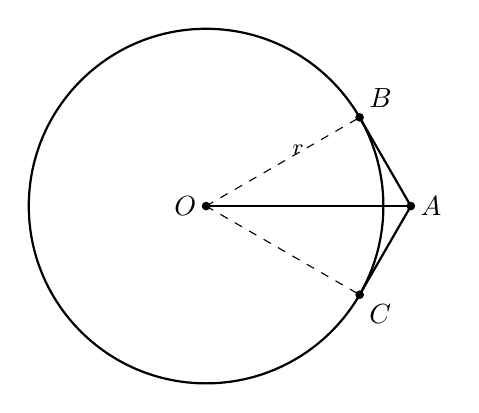
\begin{tikzpicture}[scale=1.3]
  \coordinate (O) at (0,0);
  \coordinate (A) at (2,0);
  \coordinate (B) at (1.5,0.866);
  \coordinate (C) at (1.5,-0.866);
  \draw[thick] (O) circle (1.732);
  \draw[thick] (A)--(B);
  \draw[thick] (A)--(C);
  \draw[thick] (O)--(A);
  \draw[dashed] (O)--(B);
  \draw[dashed] (O)--(C);
  \fill (O) circle (1.2pt) node[left] {$O$};
  \fill (A) circle (1.2pt) node[right] {$A$};
  \fill (B) circle (1.2pt) node[above right] {$B$};
  \fill (C) circle (1.2pt) node[below right] {$C$};
  \node at (0.9,0.55) {\footnotesize $r$};
\end{tikzpicture}
\end{center}
\nopagebreak[4]
\Needspace{4\baselineskip}
\textbf{解析}

\Needspace{5\baselineskip}
由圆外一点向圆所引两条切线长相等，且该点与圆心的连线平分两切线的夹角，故

\nopagebreak[4]
\[
\angle BAO=\frac12\angle BAC=60^\circ.
\]

\Needspace{5\baselineskip}
连 $OB$。因为半径垂直于过切点的切线，$\angle OBA=90^\circ$。在直角三角形 $OBA$ 中，

\nopagebreak[4]
\[
OB=OA\sin\angle BAO=10\sin60^\circ=10\times\frac{\sqrt3}{2}=5\sqrt3,
\]

\nopagebreak[4]
\[
AB=OA\cos\angle BAO=10\cos60^\circ=10\times\frac12=5.
\]

故 $\odot O$ 的半径为 $5\sqrt3\ \mathrm{cm}$，切线 $AB=5\ \mathrm{cm}$。

\gkanswer{答案：$\odot O$ 的半径为 $5\sqrt3\ \mathrm{cm}$，切线 $AB=5\ \mathrm{cm}$。}

\end{answer}
\begin{answer}
\gksolhead{8}{}

\textbf{题目}（10 分）：

\Needspace{5\baselineskip}
在直角 $\triangle ABC$ 中，$\angle C=90^\circ$，$CD\perp AB$。求证：

\nopagebreak[4]
\[
\frac{CD}{AD}=\frac{BD}{CD}.
\]
\nopagebreak[4]
\begin{center}% 1977 年黑龙江初试卷第 8 题：直角三角形 ABC，∠C=90°，CD⊥AB，D 为垂足，∠1=∠BCD，∠2=∠ACD（按源卷第 2 页布局）
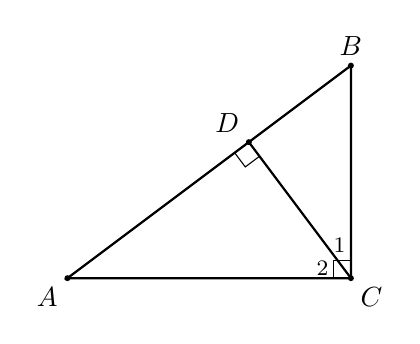
\begin{tikzpicture}[scale=0.9]
  \coordinate (A) at (0,0);
  \coordinate (C) at (4,0);
  \coordinate (B) at (4,3);
  \coordinate (D) at (2.56,1.92);
  \draw[thick] (A)--(B)--(C)--cycle;
  \draw[thick] (C)--(D);
  \draw (3.75,0)--(3.75,0.25)--(4,0.25);
  \draw (2.36,1.77)--(2.51,1.57)--(2.71,1.72);
  \fill (A) circle (1.2pt) node[below left] {$A$};
  \fill (B) circle (1.2pt) node[above] {$B$};
  \fill (C) circle (1.2pt) node[below right] {$C$};
  \fill (D) circle (1.2pt) node[above left] {$D$};
  \node at (3.84,0.47) {\footnotesize $1$};
  \node at (3.6,0.14) {\footnotesize $2$};
\end{tikzpicture}
\end{center}
\nopagebreak[4]
\Needspace{4\baselineskip}
\textbf{解析}

\Needspace{5\baselineskip}
因为 $\angle C=90^\circ$，所以 $\angle A+\angle B=90^\circ$。又因为 $CD\perp AB$，在直角三角形 $ACD$ 中 $\angle ADC=90^\circ$，故 $\angle A+\angle ACD=90^\circ$。比较两式得

\nopagebreak[4]
\[
\angle ACD=\angle B.
\]

同理，在直角三角形 $BCD$ 中 $\angle BDC=90^\circ$，$\angle B+\angle BCD=90^\circ$，结合 $\angle A+\angle B=90^\circ$ 得 $\angle BCD=\angle A$。

\Needspace{5\baselineskip}
于是 $\angle ADC=\angle CDB=90^\circ$ 且 $\angle ACD=\angle DBC$，所以

\nopagebreak[4]
\[
\triangle ADC\sim\triangle CDB.
\]

\Needspace{5\baselineskip}
对应边成比例，得 $\dfrac{AD}{CD}=\dfrac{CD}{DB}$，即

\nopagebreak[4]
\[
\frac{CD}{AD}=\frac{BD}{CD}.
\]

\gkanswer{答案：见解析版}

\end{answer}
\begin{answer}
\gksolhead{9}{}

\textbf{题目}（15 分）：

甲、乙两个车间按计划每月共生产 $450$ 件产品，粉碎“四人帮”之后，在工业学大庆运动的推动下，甲车间完成了计划的 $120\%$，乙车间完成了计划的 $110\%$，两车间共生产 $515$ 件产品，问甲、乙两车间原计划各生产多少件产品？

\Needspace{4\baselineskip}
\textbf{解析}

\Needspace{5\baselineskip}
设甲车间原计划生产 $x$ 件产品，则乙车间原计划生产 $(450-x)$ 件产品。由题意，

\nopagebreak[4]
\[
1.2x+1.1(450-x)=515.
\]

\Needspace{5\baselineskip}
两边同乘以 $10$：

\nopagebreak[4]
\[
12x+4950-11x=5150
\quad\Longrightarrow\quad
x=200.
\]

故乙车间原计划生产 $450-200=250$ 件。答：甲车间原计划生产 $200$ 件产品，乙车间原计划生产 $250$ 件产品。

\gkanswer{答案：甲车间原计划生产 $200$ 件产品，乙车间原计划生产 $250$ 件产品。}

\end{answer}
\begin{answer}
\gksolhead{10}{}

\textbf{题目}（10 分）：

计算（不查表）：

① $\sin(-510^\circ)$；

② $\left(\dfrac12\right)^{-2}-9^{\frac12}+5^0-\sqrt2\cdot\sqrt8+\log_77$。

\Needspace{4\baselineskip}
\textbf{解析}

\Needspace{5\baselineskip}
① 因为 $-510^\circ=-360^\circ-150^\circ$，正弦函数以 $360^\circ$ 为周期，故

\nopagebreak[4]
\[
\sin(-510^\circ)=\sin(-150^\circ)=-\sin150^\circ=-\sin(180^\circ-30^\circ)=-\sin30^\circ=-\frac12.
\]

\Needspace{5\baselineskip}
② 逐项计算：

\nopagebreak[4]
\[
\left(\frac12\right)^{-2}=4,\qquad
9^{\frac12}=3,\qquad
5^0=1,\qquad
\sqrt2\cdot\sqrt8=\sqrt{16}=4,\qquad
\log_77=1.
\]

\Needspace{5\baselineskip}
于是

\nopagebreak[4]
\[
\left(\frac12\right)^{-2}-9^{\frac12}+5^0-\sqrt2\cdot\sqrt8+\log_77
=4-3+1-4+1=-1.
\]

\gkanswer{答案：① $-\dfrac12$；② $-1$。}

\end{answer}
\begin{answer}
\gksolhead{11}{}

\textbf{题目}（10 分）：

在 $\triangle ABC$ 中，已知 $\angle A=120^\circ$，$\angle B=45^\circ$，$AC=6\ \mathrm{cm}$，求 $BC$ 的长。
\nopagebreak[4]
\begin{center}% 1977 年黑龙江初试卷第 11 题：△ABC 中 ∠A=120°，∠B=45°，AC=6cm（按源卷第 3 页布局）
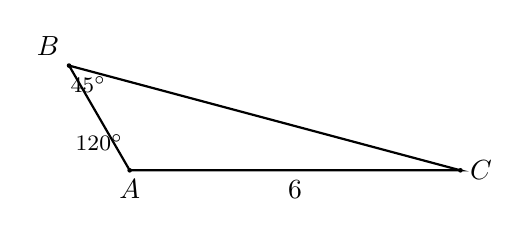
\begin{tikzpicture}[scale=0.7]
  \coordinate (A) at (0,0);
  \coordinate (C) at (6,0);
  \coordinate (B) at (-1.1,1.9);
  \draw[thick] (A)--(B)--(C)--cycle;
  \fill (A) circle (1.2pt) node[below] {$A$};
  \fill (B) circle (1.2pt) node[above left] {$B$};
  \fill (C) circle (1.2pt) node[right] {$C$};
  \node at (-0.55,0.5) {\footnotesize $120^\circ$};
  \node at (-0.75,1.55) {\footnotesize $45^\circ$};
  \node at (3,-0.35) {$6$};
\end{tikzpicture}
\end{center}
\nopagebreak[4]
\Needspace{4\baselineskip}
\textbf{解析}

\Needspace{5\baselineskip}
在 $\triangle ABC$ 中，$\angle A=120^\circ$，$\angle B=45^\circ$。由正弦定理，

\nopagebreak[4]
\[
\frac{BC}{\sin A}=\frac{AC}{\sin B}
\quad\Longrightarrow\quad
BC=\frac{AC\sin A}{\sin B}
=\frac{6\sin120^\circ}{\sin45^\circ}
=\frac{6\times\frac{\sqrt3}{2}}{\frac{\sqrt2}{2}}
=\frac{6\sqrt3}{\sqrt2}=3\sqrt6.
\]

故 $BC=3\sqrt6\ \mathrm{cm}$。

\gkanswer{答案：$BC=3\sqrt6\ \mathrm{cm}$。}

\end{answer}
\begin{answer}
\gksolhead{12}{}

\textbf{题目}（10 分）：

求函数 $y=-x^2-2x+3$ 的最大值。

\Needspace{4\baselineskip}
\textbf{解析}

\Needspace{5\baselineskip}
将 $y=-x^2-2x+3$ 配方：

\nopagebreak[4]
\[
y=-(x^2+2x)+3=-\left[(x+1)^2-1\right]+3=-(x+1)^2+4.
\]

因为二次项系数 $a=-1<0$，抛物线开口向下，函数在顶点处取最大值。当 $x=-1$ 时，$y$ 取最大值 $4$。

\gkanswer{答案：最大值为 $4$（当 $x=-1$ 时取得）。}

\end{answer}